%%%%%%%%%%%%%%%%%%%%%%%%%~~~RELATÓRIO DE MNUM TRABALHO 01-2017~~~%%%%%%%%%%%%%%%%%%%%%%%
%%%%%%%%%%%%%%%%%%%%%%%%%%%%%%%~~OBSERVATÓRIO NACIONAL~~%%%%%%%%%%%%%%%%%%%%%%%%%%%%%%%%
%%%%%%%%%%%%%%%%%%%%%%%%%%%%%~~ VICTOR RIBEIRO CARREIRA~~%%%%%%%%%%%%%%%%%%%%%%%%%%%%%%%
%------------------------------------------------------------------------------------------------------------------------------------------%
					             %MODELO DE DOCUMENTO%
%-------------------------------------------------------------------------------------------------------------------------------------------------------%
\documentclass[12pt,a4paper,final]{report}%modelo do documento tipo relatório



%-------------------------------------------------------------------------------------------------------------------------------------------------------%
										   %PACOTES UTILADOS%
%-------------------------------------------------------------------------------------------------------------------------------------------------------%
%\documentclass[border = 60pt]{standalone}
%\usepackage[landscape]{geometry}
%\usepackage{tikz}
%\usetikzlibrary{mindmap}
%\usepackage{metalogo}
%\usepackage{dtklogos}

%\documentclass[border=10pt]{standalone}

%%%%%%%%%%%%%%%%

\usepackage{tikz}
\usetikzlibrary{arrows,calc,positioning}

\tikzstyle{intt}=[draw,text centered,minimum size=6em,text width=5.25cm,text height=0.34cm]
\tikzstyle{intl}=[draw,text centered,minimum size=2em,text width=2.75cm,text height=0.34cm]
\tikzstyle{int}=[draw,minimum size=2.5em,text centered,text width=3.5cm]
\tikzstyle{intg}=[draw,minimum size=3em,text centered,text width=6.cm]
\tikzstyle{sum}=[draw,shape=circle,inner sep=2pt,text centered,node distance=3.5cm]
\tikzstyle{summ}=[drawshape=circle,inner sep=4pt,text centered,node distance=3.cm]
%%%%%%%%%%%%%%%%%%%%%%%%%
\usepackage{smartdiagram}
\usepackage[utf8x]{inputenc}
\usepackage{ucs}
\usepackage{multicol}
\usepackage[comma,authoryear]{natbib}%citação com parentesis e autor ano
\usepackage[english, brazil]{babel}
\usepackage{amsmath}
\usepackage{amsfonts}
\usepackage{amssymb}
\usepackage[colorlinks = true, linkcolor = blue, urlcolor  = blue, citecolor = blue, anchorcolor = blue]{hyperref}
\usepackage{indentfirst}
\usepackage{setspace}
\usepackage{makeidx}
%\usepackage[table]{xcolor}
\usepackage{graphicx}
\usepackage{color}
\usepackage{lipsum} % Required to insert dummy text. To be removed otherwise
\usepackage{epstopdf}%adiciona imagens em formato eps no pdf.
\usepackage{subfigure}%cria ambientes de multifiguras
\usepackage{float}%coloca as figuras exatamente aonde você quer
%\usepackage[monochrome]{xcolor}%imprime o arquivo final em preto e branco
\usepackage[left=2cm,right=2cm,top=2cm,bottom=2cm]{geometry}
\usepackage{lipsum} % Required to insert dummy text. To be removed otherwise
\usepackage{multicol, blindtext, graphicx}%cria figura na página inteira
\usepackage{booktabs} % To thicken table lines
\usepackage{tikz}%pacote para fazer fluxogramas
\usepackage{verbatim}%
\usetikzlibrary{calc,trees,positioning,arrows,chains,shapes.geometric,decorations.pathreplacing,decorations.pathmorphing,shapes,matrix,shapes.symbols}
\author{Victor Ribeiro Carreira}
\title{Projeto de Doutorado 2016}


%--------------------------------------------------------------------------------------------------------------------------------------------------------%
								%INÍCIO DO RELATÓRIO%
%--------------------------------------------------------------------------------------------------------------------------------------------------------%

\begin{document}
\thispagestyle{empty}% retira a numeração da primeira página


\begin{figure}[H]
\centering
\subfigure{
\includegraphics[scale=1.3]{Imagens/logoON.jpg}}
%\subfigure{
\includegraphics[scale=1.5]{Imagens/logoMCT.png}}
\end{figure}

\vspace{1cm}

\begin{center}
\textbf{MODELAGEM NUMÉRICA DE ONDAS SÍSMICAS}
\end{center}

\vspace{3cm}

\begin{center}
\textbf{RELATÓRIO $01$:} DIFERENÇAS FINITAS EM UM REGIME TRANSIENTE $1$D EM UMA BARRA POR MEIO DA FORMULAÇÃO EXPLÍCITA.
\end{center}

\vspace{2.5cm}

\begin{center}
\textbf{PROFESSOR:} LEANDRO DI BARTOLO
\end{center}

\begin{center}
\textbf{ALUNO:} VICTOR RIBEIRO CARREIRA
\end{center}

\vspace{10cm}

\begin{center}
- 2017 -
\end{center}


%--------------------------------------O relatório---------------------------------------------------

\pagebreak%
\setstretch{1.5}
\section*{Introdução}

O estudo da energia em trânsito na forma de calor compreende uma das áreas mais fundamentais da ciência e é apresentado como foco principal deste relatório. Os problemas que envolvem transferência térmica causada por diferenças de temperatura entre duas ou mais regiões podem ser descritos por equações diferenciais parciais. Estas determinam a temperatura em qualquer lugar ou momento de um objeto de estudo e são denominadas equações de calor. 

As equações diferenciais são em grande parte primordiais para modelar a maioria dos fenômenos naturais. Com elas podemos determinar o comportamento futuro de diversos problemas com base na variação dos valores presentes. Contudo, a resolução de equações diferenciais parciais pode ser complexa dificultando a obtenção de soluções exatas por meio dos métodos analíticos existentes.

Os métodos numéricos resolvem essa lacuna de soluções analíticas complexas. Este conjunto de métodos reduzem um problema contínuo, com um número infinito de soluções, em um problema discreto, com um número finito de variáveis, que possui uma solução computacional. Este processo de \textit{discretização} é utilizado em diversos métodos numéricos, tais como: o método das diferenças finitas, método dos volumes finitos, método dos elementos de contorno, e, o método dos elementos finitos \citep{Melo2011}.

Este relatório aborda somente o método das diferenças finitas explícito para um caso unidimensional.  


\section*{Objetivo}

O objetivo deste trabalho é analisar a transferência de calor no decorrer do tempo em dois problemas que envolvem condução de calor unidimensional em uma barra. 

O primeiro deles é reproduzir o exemplo mostrado, em aula, onde uma barra é discretizada com 6 pontos. Rodando tempo suficiente para encontrar a solução de equilíbrio. E comparar esses resultados qualitativamente com os resultados mostrados, no exemplo de aula.

O segundo é aumentar o número de pontos na direção espacial $x$ (diminuindo o espaçamento $\Delta x$), mantendo o mesmo problema físico. Ou seja, tanto as dimensões quanto as propriedades físicas devem permanecer as mesmas. O critério de estabilidade numérica $\lambda \leq \frac{1}{2}$, escolhendo um intervalo de tempo $\Delta t$ apropriado. O $\lambda$ adotado dever ser igual ao do item anterior.

E, por final, comparar a diferença entre os erros obtidos entre as duas soluções numéricas, obtidas pelo método das diferenças finitas na forma explícita, com a solução analítica.


\section*{Fundamento teórico}
\subsection*{A equação do calor}

A equação difusão de calor é uma equação diferencial parcial parabólica \footnote{Dada EDP linear na forma genérica: $ A \frac{\partial^{2} u} {\partial x^{2}} + B \frac{\partial^{2} u }{\partial x \partial y} + C \frac{\partial^{2} u} {\partial y^{2}} + D \frac{\partial u}{\partial x} + E \frac{\partial u}{\partial y} + Fu = G(x,y)$ denomina-se parabólica quando o termo $\Delta=B^{2}-4 A C=0$.} de segunda ordem. Esta equação determina o campo de temperaturas em um dado meio. A relação física fundamental descrita por esta equação é dada pelo equilíbrio da taxa de calor que entra, em qualquer parte de um corpo, é igual a taxa de absorção de calor naquela parte do corpo, seja este $1$D, $2$D ou $3$D.

A equação fundamental pode ser expressa da forma (Eq. \ref{calor})

\begin{equation}
\frac{\partial}{\partial x} (k \frac{\partial u}{\partial x}) + \frac{\partial}{\partial y} (k \frac{\partial u}{\partial y}) + \frac{\partial}{\partial z} (k \frac{\partial u}{\partial z})+ \dot{q} = \rho s \frac{\partial u}{\partial t}
\label{calor}
\end{equation}

Onde:

$k$, condutividade térmica ($W/mK$)

$\rho$, densidade ($Kg/m$)

$s$, calor específico do material ($J/kg K$)

$u$, temperatura ($K$)

$\dot{q}$, é a taxa na qual a energia é gerada por undidade de volume no meio ($W/m$)


A solução da Eq. \ref{calor} gera um campo de temperaturas $u=u(x,y,z,t)$. No caso $1$D, este campo pode ser descrito como $u=u(x,t)$. Portanto a Eq. \ref{calor} pode ser reescrita como:

\begin{equation}
\frac{\partial}{\partial x} (k \frac{\partial u}{\partial x}) + \dot{q} = \rho s \frac{\partial u}{\partial t}
\label{calor2}
\end{equation}

No caso em que não há uma taxa de geração de energia associada à taxa de geração de energia o termo $\dot{q}=0$, logo a Eq. \ref{calor2} poder ser descrita de acordo com a Eq \ref{calor3}. 


\begin{equation}
\frac{\partial}{\partial x} (k \frac{\partial u}{\partial x}) = \rho s \frac{\partial u}{\partial t}
\label{calor3}
\end{equation}

Ao se considerar a condutividade térmica $k$ constante a Eq. \ref{calor3} pode ser reescrita conforme a Eq. \ref{calor4}


\begin{equation}
\alpha^{2} \frac{\partial^{2} u}{\partial x^{2}} = \frac{\partial u}{\partial t}
\label{calor4}
\end{equation}

Onde $\alpha^{2}$ é a difusividade térmica que é um parâmetro que depende apenas do material da barra e seus valores são tabelados em unidades de comprimento por tempo\footnote{Observação:$ \alpha^{2}\left[\frac{L^{2}}{T}\right]$}.

\subsection*{Diferenças finitas progressivas}


A ideia primordial do método das diferenças finitas é transformar a resolução de equações diferenciais em um sistema de equações algébricas substituindo as derivadas por diferenças \citep{Melo2011}. Ou seja, a equação diferencial que se deseja aproximar pode ser numericamente equilibrada em cada ponto discreto do modelo. Assim, o domínio é discretizado através de uma malha regularmente espaçada em cada uma das dimensões do problema, sendo as funções e propriedades de interesse consideradas apenas nestes pontos discretos \citep{Bartolo2010}.

No caso de uma barra $1$D, a discretização segue de acordo com o esquemático apresentado na Fig. \ref{Discretizacao}.

\begin{figure}[H]
\centering
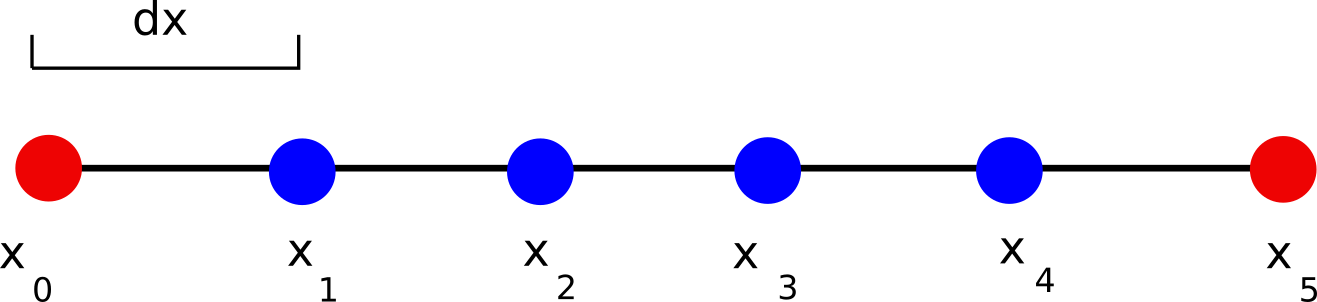
\includegraphics[scale=1]{Imagens/Discretizacao1d.png}
\caption{Discretização de uma malha unidimensional com espaçamento constante $dx$. Os pontos vermelhos representam pontos com temperatura constante e conhecidas e os pontos azuis representam os pontos com as temperaturas a serem determinadas.}
\label{Discretizacao}
\end{figure}

A Fig. \ref{DF} apresenta a definição geométrica de uma derivada por diferença finita progressiva em comparação com a derivada analítica.

\begin{figure}[H]
\centering
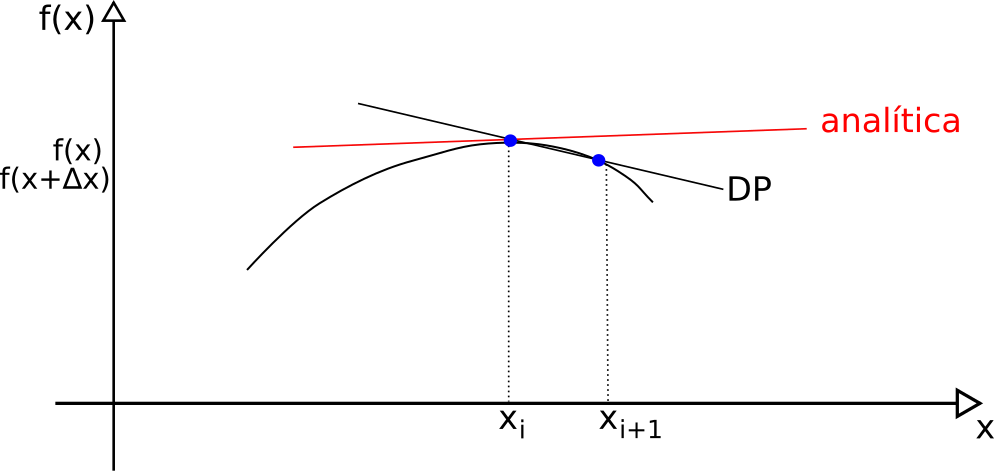
\includegraphics[scale=1.2]{Imagens/DP.png}
\caption{DP - Diferença Finita Progressiva}
\label{DF}
\end{figure}


Considerando $f(x)$ e suas derivadas como funções contínuas pode-se expandir a função através da série de Taylor em torno do ponto $x_{i}$, através da seguinte da Eq. \ref{Taylor}.

\begin{equation}
f(x)=\sum^{\infty}_{n=0}\frac{1}{n!}\frac{d^{n}f(x)}{dx^{n}|_{x=x_{0}}}(x-x_{0})^{n}
\label{Taylor}
\end{equation}

Onde a variável $x$ pode ser considerada tanto uma variação temporal quanto espacial.








\section*{Resultados}
\subsection*{Caso I}

\subsection*{Caso II}



\section*{Discussão dos resultados}


%exemplo de tabela
%\begin{table}[]
%\centering
%\caption{Compilação de Perfis usados na inferência de litologia.}
%\label{rock-properties}
%\begin{tabular}{@{}llllllllll@{}}
%\toprule
%Rocha         & Densidade ($g/cm^{3}$) & Raios-Gama ($Ci/g$)& Potencial-Espontâneo ($mV$)&   \\ \midrule
%Conglomerado &     $2,50$  &       ---        &    ---        &      \\
%Arenito  &    $2,35$      &       $2,00\leftrightarrow4,00$       &     ---       &      \\
%Folhelho &   $2,40$       &      ---        &      ---      &    \\
%Argilito &     $2,55$   &          ---     &       ---     &     \\
%Siltito  &      $2,21$    &          ---     &       ---     &   \\
%Dolomita &     $2,70$    &        $8,00$       &   ---         &       \\
%Marga  &    $2,50$     &         ---      &    ---        &     \\
%Basalto  &     $2,99$    &          $0,50$     &    ---       &      \\
%Diabásio &    $2,90$    &         ---      &       ---     &     \\
%Lava &     $2,61$    &      $0,33$         &      ---      &      \\
%Granito &    $2,64$      &       $0,70\leftrightarrow4,80$        &      ---      &      \\
%Gabro &    $3,03$     &       ---        &     ---       &       \\
%Peridotito &   $3,15$    &      ---         &     ---       &      \\
%Quartzito &    $2,60$    &        $5,00$      &     ---       &    \\
%Xisto &   $2,64$    &         ---      &      ---      &    \\
%Gnaisse &    $2,80$     &      ---         &    ---        &        \\
%Serpentinito &    $2,78$     &   ---            &   ---     &        \\
%Anfibolito &  $2,96$       &          ---     &       ---     &        \\
%Eclogito &  $3,37$    &       ---        &      ---      &    \\
%Mármore &   $2,75$       &      ---         &     ---       &      \\ \bottomrule
%\end{tabular}
%\end{table}



%-----------------------------------Bibliografia-------------------------------------------------%
%\chapter{Referências}
\bibliographystyle{apalike}
\bibliography{referencias.bib}

\end{document}
